\chapter{Kubernetes}

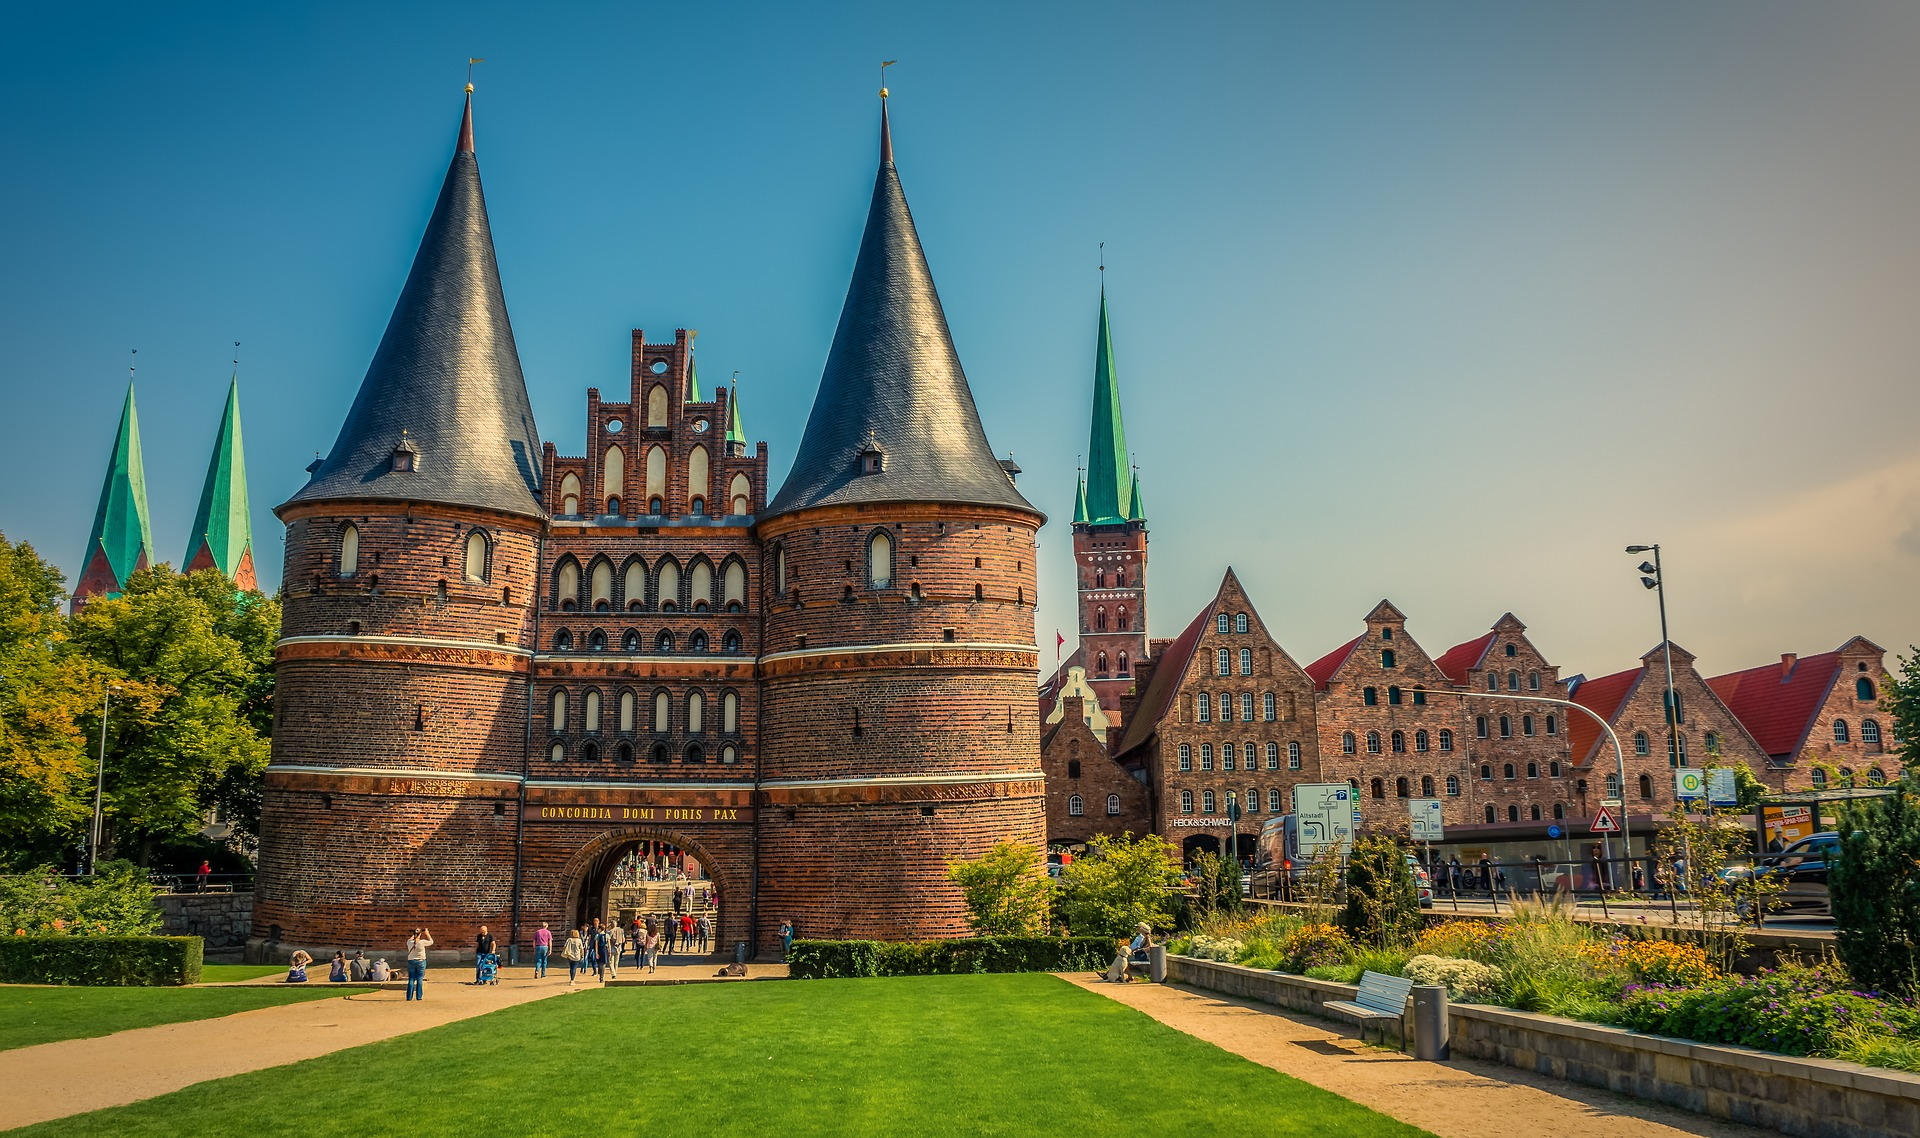
\includegraphics{45-kubernetes.jpg}

\justifying
By now you've probably at least heard the word Kubernetes, and may have some familiarity with it. At it's
simplest, Kubernetes\index{Kubernetes} is a framework for managing deployments at scale. By putting our
workloads and applications into container images, we can move our code from inception, through the build pipeline
and on to deployments and container registries with ease. Although the learning curve can feel steep at times,
learning this new way of working can give a considerable boost to efficiency and productivity.

\section{Working with Kubernetes}

\justifying
The Kubernetes environment is implemented in ``clusters''. Clusters can be divided into logical partitions known
as ``namespaces''.

\subsection{Public Cloud and Kubernetes}

\justifying
The most well known of the public cloud providers offer services to ease the creation of Kubernetes clusters.

\section{Command Line Tools}

